\documentclass{article}
\PassOptionsToPackage{numbers,sort&compress}{natbib}
\usepackage[dblblindworkshop,final]{neurips_2026}
\workshoptitle{Foundations of Agentic Systems Theory}

\usepackage[utf8]{inputenc} % allow utf-8 input
\usepackage[T1]{fontenc}    % use 8-bit T1 fonts
\usepackage{hyperref}       % hyperlinks
\hypersetup{
  pdftitle={Nudging the Graph, Not the Agent: A Benchmark for Alignment by Environment Design},
  pdfauthor={Yuriy Dementiev},
  pdfsubject={FAST Workshop at NeurIPS 2026},
  hidelinks
}
\usepackage{url}            % simple URL typesetting
\usepackage{needspace}
\usepackage{booktabs}       % professional-quality tables
\usepackage{amsfonts}       % blackboard math symbols
\usepackage{nicefrac}       % compact symbols for 1/2, etc.
\usepackage{microtype}      % microtypography
\usepackage{xcolor}         % colors

\usepackage{tikz}
\usetikzlibrary{arrows.meta,positioning}

\newcommand{\MCTA}{\textsc{Minimum-Cost Task Alignment}}
\newcommand{\tw}{\mathrm{tw}}

% Note. For the workshop paper template, both \title{} and \workshoptitle{} are required, with the former indicating the paper title shown in the title and the latter indicating the workshop title displayed in the footnote.
\title{Nudging the Graph, Not the Agent:\\
       A Benchmark for Alignment by Environment Design}


\author{Yuriy Dementiev\\
ITMO University}

\begin{document}


\maketitle

\begin{abstract}
Agent harnesses are environments: the tools on offer, the ordering of steps and
the presence of shortcuts determine not only what an agent \emph{can} do but what
it \emph{will} do. Practitioners already align agents by editing these
environments---removing a tool, forcing a checkpoint, blocking a shortcut---without
a formal objective, a solver, or any guarantee that an edit constrains
\emph{every} trajectory the agent might sample. The Kleinberg--Oren model of
present-biased planning on task graphs provides a formal model of this setting, and the
accompanying \MCTA{} problem asks for the cheapest edit forcing every feasible
trajectory under the model to reach the goal and perform prescribed critical actions. The
theory is well developed and has never been executed. We release NudgeBench: 18\,045
task graphs from four source corpora spanning three domains---agent tool
decompositions, university curricula and scientific workflow traces---
annotated with the structural parameters that govern tractability; six parametric
instance families whose decision thresholds are placed analytically; exact and
heuristic solvers; and an agent-in-the-loop probe that computes the exact interval
of discount factors consistent with observed choices under the model. Real task graphs turn out structurally
narrow---treewidth in single digits where prior measurements of network data report
hundreds---yet two of seven workflow families remain intractable regardless,
because tractability turns on weight diversity as much as on width. The repair an
engineer would make by hand matches the optimum on the median real instance and
costs up to $2.67\times$ more in the tail, on instances of treewidth two. On
the tested general graphs, choices are consistent with little or no present bias
under the model. In deferral traps---a large step toward the goal beside cheap ways
of postponing it---one model repeatedly defers and another does not. This behaviour
is consistent with present-biased planning but does not uniquely identify its
mechanism. Separately, theory-derived edits increase compliance from $0/240$ to
$240/240$ observed rollouts, despite a mismatch between the design discount factor
and the probe's interval. These observations do not establish guarantees for
arbitrary stochastic agents.
Code is available at \mbox{\url{https://github.com/yudementiev/NudgeBench}}.
\end{abstract}

\section{Introduction}

Designing an agent's harness is already alignment work. Which tools are exposed,
which steps are mandatory, whether a cheap shortcut sits beside the thorough
route---these choices shape the actions available to an agent, and
practitioners make them constantly. They make them by intuition. There is no
objective being minimised, no solver, and no way to check that an edit binds every
trajectory the agent might produce rather than the one it happened to produce
during testing.

A formal account exists. Kleinberg and Oren~\cite{kleinberg2014} model an agent
traversing a task DAG that evaluates plans under a present-biased discount: the
next action counts in full, everything after it is discounted by $\beta$. Such an
agent can announce a sensible plan and abandon it on arrival, with nothing about
the environment having changed in between. The principal cannot alter $\beta$ but
can edit the graph, and \MCTA{}~\cite{belova2024,belova2026} asks for the cheapest
edit forcing every feasible trajectory to reach the target and traverse a
prescribed set of critical arcs.

This line has produced a detailed complexity landscape and no experiments. Nobody
has run the algorithms, measured the environments they assume, or checked the
behavioural premise against an actual agent. Each needs a benchmark that does not
exist: instances real enough to say something about deployment, annotated with the
parameters the theory is stated in, and solvers trustworthy enough to compare
against.

The guarantee applies to all feasible trajectories \emph{under the planning
model}. Stochastic LLM sampling is not generally equivalent to arbitrary
tie-breaking among model-optimal actions: an LLM may select a strictly worse action.
We therefore distinguish three questions: structural measurements characterise the
tasks, behavioural probes assess consistency with the model, and intervention
experiments measure the empirical effectiveness of graph edits. The last does not
by itself validate the behavioural model or extend its guarantee to arbitrary LLM
policies.

\section{Setting}

An instance is $M = (G, w, s, t, \beta, r)$ with $G$ a weighted DAG. Standing at
$v$, the agent evaluates every $v$--$t$ path under
\[
  \zeta(P) \;=\; w(e_1) + \beta \sum_{i \geq 2} w(e_i),
\]
abandons if $\min_P \zeta(P) > \beta r$, and otherwise commits to $e_1$ and
repeats. Ties are broken arbitrarily, so the model induces a \emph{set} of feasible
trajectories rather than a single path. \MCTA{} seeks $S \subseteq E$ minimising
$\sum_{e \in S} c(e)$ such that in $G - S$ every feasible trajectory reaches $t$ and
traverses every arc of $T$. Costs are real-valued, so an auxiliary arc with a
negative deletion cost is one the solver pays to \emph{keep}: a single objective
carries both deletion and paid addition. Figure~\ref{fig:example} shows why blocking
the tempting route is not generally enough.

\begin{figure}[t]
\centering
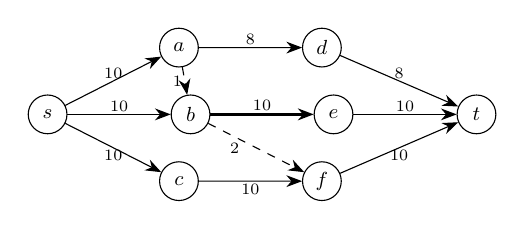
\begin{tikzpicture}[
  scale=0.82, transform shape,
  >={Stealth[length=2mm]},
  every node/.style={font=\small},
  st/.style={circle,draw,minimum size=6mm,inner sep=0pt},
  w/.style={font=\scriptsize,inner sep=1pt}
]
\node[st] (s) {$s$};
\node[st,above right=6mm and 16mm of s] (a) {$a$};
\node[st,right=16mm of s]              (b) {$b$};
\node[st,below right=6mm and 16mm of s] (c) {$c$};
\node[st,right=16mm of a] (d) {$d$};
\node[st,right=16mm of b] (e) {$e$};
\node[st,right=16mm of c] (f) {$f$};
\node[st,right=16mm of e] (t) {$t$};

\draw[->] (s) -- node[w,above]{10} (a);
\draw[->] (s) -- node[w,above]{10} (b);
\draw[->] (s) -- node[w,below]{10} (c);
\draw[->] (a) -- node[w,above]{8}  (d);
\draw[->] (c) -- node[w,below]{10} (f);
\draw[->] (d) -- node[w,above]{8}  (t);
\draw[->] (f) -- node[w,below]{10} (t);
\draw[->] (e) -- node[w,above]{10} (t);

\draw[->,very thick] (b) -- node[w,above]{10} (e);
\draw[->,dashed] (b) -- node[w,pos=0.35,below left]{2} (f);
\draw[->,dashed] (a) -- node[w,left]{1} (b);
\end{tikzpicture}
\caption{The worked example, after~\cite{belova2026}. With $\beta = 1/2$ and
$r = 36$ the agent walks $sbft$, skipping the critical arc $(b,e)$ (thick).
Deleting the shortcut $(b,f)$ only diverts it to $sadt$, which also skips $(b,e)$;
adding the auxiliary arc $(a,b)$ yields $sabet$. Our simulator reproduces every
perceived cost the paper states, and those numbers are the test suite.}
\label{fig:example}
\end{figure}

\section{NudgeBench}
\label{sec:bench}

The benchmark has three parts: instances derived from published data, instance
families generated to a specification, and the tooling that makes both measurable.

\subsection{A taxonomy of instances}

\begin{table}[t]
\caption{What each domain of origin supplies. \emph{Branching} counts instances
with any node offering a choice of continuation; fan-in---several inputs to one
task---is not a decision. \emph{Discriminating} counts those on which a patient and
a biased agent walk different routes, which is the only kind that can measure an
agent at all. Reproduce with \texttt{scripts/taxonomy.py}.}
\label{tab:corpus}
\centering
\small
\begin{tabular}{llrrrrr}
\toprule
Domain of origin & Source & Instances & Branching & Discrim. & Arcs (med.) & $\tw$ \\
\midrule
\multicolumn{7}{l}{\emph{Agent task decompositions} --- synthetic weights} \\
\quad everyday APIs   & TaskBench~\cite{taskbench} & 4\,318 &   275 &   0 & 2--9 (4)     & 2 \\
\quad multimedia      & TaskBench                  & 5\,548 &   525 &  21 & 2--11 (4)    & 2 \\
\quad HuggingFace     & TaskBench                  & 7\,435 &   775 &  42 & 2--11 (4)    & 2 \\
\midrule
\multicolumn{7}{l}{\emph{Human curricula} --- synthetic weights} \\
\quad Caltech         & \cite{stavrinides2023}     &   169 &   169 &  28 & 7--30 (14)   & 4 \\
\quad Johns Hopkins   & \emph{ibid.}, from prose   &   533 &   495 & 119 & 6--180 (23)  & 6 \\
\midrule
\multicolumn{7}{l}{\emph{Scientific workflows} --- \textbf{measured runtimes}} \\
\quad montage         & WfCommons~\cite{wfcommons} &     6 &     6 &   5 & 130--1336 (365) & 18 \\
\quad soykb           & WfCommons                  &     6 &     6 &   2 & 202--757 (479)  & 12 \\
\quad five others     & WfCommons                  &    30 &    30 &   1 & 42--1201        & 2--3 \\
\bottomrule
\end{tabular}
\end{table}

Table~\ref{tab:corpus} is the benchmark's central artefact, and its middle columns
carry a result. \textbf{The domain agents actually operate in barely produces
environments that can pose the question.} Of 17\,301 agent task decompositions,
1\,575 contain any choice of continuation and 63 are discriminating; the everyday
API domain contains none whatsoever. Their dependency structure is overwhelmingly
fan-in, and their graphs are tiny---a median of four arcs, treewidth two. Human
curricula, designed by people for people, are markedly richer: 147 discriminating
instances from 702, reaching 180 arcs. Scientific workflows are the largest graphs
in the corpus by an order of magnitude and yield 8 discriminating instances from 42,
because their parallel fan-out routes are interchangeable.

Two consequences shape how the benchmark should be used. Domain of origin predicts
structure far better than instance count does, so pooling these sources would report
an average describing none of them. And parametric families are not padding beside
real corpora but a necessary complement, supplying on demand the choice structure
the real data does not contain.

\subsection{Instances from published data}

\textbf{Agent task decompositions.} TaskBench~\cite{taskbench} publishes user
requests decomposed into tool calls, with the dependency between calls annotated and
each record labelled by its own topology---a single call, a chain, or a branching
DAG. Three tool domains ship. An instance is the decomposition bracketed between a
virtual source and sink, charging each arc the cost of the call it enters. This is
the only corpus here drawn from agent tasks rather than human ones, which is what
makes its emptiness in Table~\ref{tab:corpus} informative rather than merely
disappointing.

\textbf{Course-prerequisite networks.} An instance is the \emph{prerequisite
closure} of a target course---everything that can reach it, plus a virtual source
joined to the entry points---so a path is one order in which a student could arrive
there. Closures of at least six courses and depth three are kept: Caltech yields 169
from 771 courses, Johns Hopkins 533 from 10\,075.

One mapping decision limits every corpus here and we state it rather than bury it:
dependency graphs are \emph{conjunctive}---a task needs all its inputs---while an
agent path is a \emph{sequence}. An instance therefore answers ``how hard is this
shape to align'', not ``what should this student enrol in''. Johns Hopkins adds a
second: it has no cleaned prerequisite column, only catalogue prose, so course codes
are extracted by pattern. Two blurbs in five express a disjunction that this reading
turns into a conjunction, which only \emph{adds} arcs---the safe direction, since
treewidth never falls when arcs are added, so its figures bound the real curriculum
from above.

\textbf{Scientific workflows.} WfCommons publishes traces of production runs
recording both the dependency graph and how long each task took: 42 traces across
seven applications, 22 to 601 tasks. These are the only instances whose weights are
\emph{measured}, which matters beyond realism---Section~\ref{sec:c1} shows those
continuous runtimes deciding tractability as much as topology does.

\subsection{What makes an instance measure anything}
\label{sec:discriminating}

Most instances are useless for probing an agent, and quietly so. If every route
costs the same, or one dominates at every discount factor, a patient planner and a
heavily biased one produce the same trajectory; reporting such an episode as evidence
of patience would be an error, and pooling many would swamp the informative ones.
NudgeBench therefore marks an instance \emph{discriminating} when $\beta = 1$ and
$\beta = 0.4$ walk different routes, and the agent experiments draw only from those.
We report the filter rather than only its output, because the same corpus filtered
differently supports different conclusions.

Curriculum data carries no workload column, so weights on those instances are drawn
from a small integer palette $\{2,3,5,8,13\}$. This is an assumption, not a
measurement. Whole numbers are deliberate: the probe asks an agent to total its own
route as an arithmetic control, and awkward decimals would confuse ``cannot add''
with ``cannot add \emph{this}''.

\subsection{Generated families}

Six parametric families cover what real instances cannot supply on demand: a
decision threshold placed exactly where an experiment needs it.

\textbf{Calibrated two-route traps.} One route is cheap now and dear later, the
other splits its cost evenly; solving
$\textit{immediate} + \beta \cdot \textit{tail} \le 2\,\textit{steady}$ for the tail
places the flip at any chosen $\beta$. An \emph{integer} variant searches whole-number
triples, since asking a model to total $13.993$ tests the wrong thing; a \emph{deep}
variant stretches each route into a chain, so comparing them means summing several
numbers rather than one.

\textbf{Compliance families.} Present bias hurts in two distinguishable ways, and
Figure~\ref{fig:example} is the second: the tempting route is also the
\emph{cheapest}, so nothing is wasted and only compliance fails. Matching both
routes' totals forces the threshold to $1$ by algebra---any bias at all
defects---giving the most sensitive detector available at the cost of not localising
$\beta$; putting the required action on a route dearer outright means no $\beta$
complies unaided and only editing the environment helps.

\textbf{Deferral traps.} A node offers one large arc straight to the target and
several cheap arcs leading to nodes offering \emph{the same choice again}. Deferring
is preferred exactly when $\beta < 1 - \textit{small}/\textit{big}$, so the ratio
sets the threshold. Because the next node is identical, an agent below the threshold
defers repeatedly: the number of deferrals measures how far procrastination runs,
which no two-route trap can ask. This family was not designed from the theory---
Section~\ref{sec:deferral} describes where it came from.

\textbf{Structural families.} Layered fan-out/fan-in, independent parallel
pipelines, and series-parallel nesting, after the shapes catalogued for scientific
workflows~\cite{bharathi}. Series-parallel composition keeps treewidth at most two,
which is the regime where MCTA is already NP-hard, so those instances are where a
small structural parameter provably fails to rescue the problem.

\subsection{Annotation, solvers, and release}

Every instance carries the parameters Theorem~8 of~\cite{belova2026} is stated in:
treewidth, pathwidth, vertex cover, feedback vertex set, longest path $p$, distinct
arc weights $|W|$, and the distinct path weights $|L|$ the dynamic program is
exponential in. The three NP-hard ones are \emph{certified intervals} rather than
points---treewidth floored by minor-min-width, capped by the better of two
elimination heuristics, each exhibiting a real decomposition---because ``at most 6''
is sound whatever the truth and ``is 6'' is not. Two solvers ship: an exact branch
and bound reporting whether optimality was proved or the budget ran out, validated
against an independent brute force written in the tests rather than the library, and
a witness-guided heuristic rendering the engineer's move as an algorithm. Released
with them: the four corpora as loaders (data fetched from its authors, not vendored),
the generators, the structural measurement, the agent probe, and the full transcript
of every API call made for this paper, so any number can be re-scored without
re-spending. The 179 tests assert claims rather than absence of crashes and run under
three hash seeds, for reasons Appendix~\ref{app:cost} makes clear.

\section{Environments are narrow, and that is not enough}
\label{sec:c1}

\begin{table}[t]
\caption{Structural parameters, reproducible with \texttt{scripts/census.py}. Every
NP-hard quantity is a certified interval, not a point estimate.}
\label{tab:structure}
\centering
\begin{tabular}{lccc}
\toprule
Graph & Treewidth & $p$ & $|L|$ \\
\midrule
Caltech, largest component (436 nodes, 747 arcs) & 8--12 & --- & --- \\
Caltech, 169 instances            & median 3, max 5  & max 7  & max 8 \\
Johns Hopkins, largest component (665, 1708) & $\leq 25$ & --- & --- \\
Johns Hopkins, 533 instances      & median 3, max 11 & max 12 & max 13 \\
\midrule
seismology, 601 tasks             & \textbf{2}      & 3  & 415 \\
epigenomics, 233 tasks            & \textbf{2}      & 10 & 286 \\
soykb, 336 tasks                  & \textbf{12}     & 12 & 6\,610 \\
montage, 472 tasks                & \textbf{17--18} & 9  & 34\,986 \\
\bottomrule
\end{tabular}
\end{table}

The motivating claim survives: task graphs are narrow, against the hundreds Maniu
et al.~\cite{maniu2019} report for database and road networks. The contrast is worth
drawing precisely because their corpus is network data rather than task graphs, so
structural narrowness appears to be a property of the latter specifically.

The second half is the interesting one. The dynamic program of~\cite{belova2026}
runs in $(|L|+1)^{O(\tw)}$ time, so width alone does not decide feasibility. Montage
reaches $10^{81}$ states and its treewidth \emph{grows with problem size}, from 5 at
58 tasks to 18 at 472; soykb reaches $10^{46}$. Five of seven workflow families are
trivially tractable and two are hopeless. \textbf{A graph can be narrow and still out
of reach.} This argues for the theorem's form rather than against it, and gives the
open question of whether an $f(\tw) \cdot m^{g(p)}$ algorithm exists a concrete
constituency: montage has $p = 9$ at every size, so such an algorithm would rescue
exactly the family the current one cannot.

One practical lever falls out. Rounding runtimes to whole seconds collapses $|L|$
from $34\,986$ to $385$ in montage and barely moves srasearch. The principal's unit
of account is a design parameter of the intervention, not an implementation detail.

\section{The intuitive repair is usually right and occasionally expensive}
\label{sec:c2}

\begin{table}[ht]
\centering
\begin{tabular}{lrrrr}
\toprule
Corpus & Solved & Optimality proved & Heuristic worse & Worst ratio \\
\midrule
Caltech                        & 65 & 65 & 10 & $\mathbf{2.00\times}$ \\
Johns Hopkins ($\leq 28$ arcs) & 87 & 74 &  2 & $\mathbf{2.67\times}$ \\
\bottomrule
\end{tabular}
\caption{Witness-guided heuristic against the exact optimum on real instances.}
\label{tab:solvers}
\end{table}

The heuristic's median cost ratio against the exact optimum is $1.00$: usually the
local fix is simply correct. The tail is where it is not, and the instances where it
loses have \textbf{treewidth 2--3}. Being narrow does not make the greedy choice
right. Exact solving takes milliseconds on the median instance and seconds in the
tail; the search budget runs out between 20 and 28 arcs, which is where hardness
begins to bite in practice.

\section{Agents}
\label{sec:agents}

\subsection{The probe}

Each episode puts one agent through two conditions on one instance: state a complete
route, then walk it one committed action at a time. The agent sees the whole graph in
both---present bias is discounting the future, not being blind to it. Labels are
re-randomised every episode, since the worked example of~\cite{belova2026} is
published and a model recognising it would be reciting rather than deciding.

The probe computes the exact interval of discount factors consistent with observed
choices under the model. Choosing $e^\ast$ over $e$ requires
$w(e^\ast) + \beta\, d(\mathrm{head}(e^\ast)) \leq w(e) + \beta\, d(\mathrm{head}(e))$,
a linear inequality in $\beta$; intersecting these inequalities across a run gives
the compatible interval. An empty intersection rejects a common discount factor
under these choice constraints. A nonempty interval establishes consistency, not a
unique internal discount factor or the mechanism generating the choices.

The agent also totals its stated route as an arithmetic control. Passing this
control does not exclude local-cost heuristics or planning errors. Every failure to
produce a move is classified by cause: token ceiling, provider content filter,
empty response, or unparseable response, keeping harness failures separate from
behavioural observations.

\subsection{Little evidence of present bias on general graphs}

\begin{table}[ht]
\caption{Discriminating prerequisite closures of 8--26 arcs, presented in full. The
arithmetic control passes throughout; the intervals describe model consistency,
not uniquely identified behavioural mechanisms.}
\label{tab:agents}
\centering
\begin{tabular}{lrrrl}
\toprule
Model & Episodes & Arithmetic & Optimal route & $\beta$ \\
\midrule
\texttt{claude-opus-5}      & 40 & 100\% &  98\% & $[1.000,\,1]$ \\
\texttt{gemini-3.7-flash}   & 40 & 100\% & 100\% & $[0.846,\,1]$ \\
\texttt{deepseek-v4-flash}  &  8 & 100\% &  88\% & $[1.000,\,1]$ \\
\bottomrule
\end{tabular}
\end{table}

Calibrating instances to the human effort-discounting band $\beta \in [0.70,
0.79]$~\cite{augenblick,cheung} proved useless: every agent sat above it, and traps
had to be rebuilt up to $\beta = 0.99$ before they bracketed anything. On the
strongest of those---one hour of work now against 118 later, versus 59 and
59---\texttt{gemini-3.7-flash} took the steady route in 100 of 100 episodes. Telling
the agent that the future is uncertain, in a framing that discounts the reward by the
same mechanism, did not change this either.

These observations provide little evidence of present bias on the tested general
graphs. Both lower-cost and frontier models choose largely patient routes in this
setting; this comparison does not isolate the effect of reasoning budget.

\subsection{Repeated deferral in a specific configuration}
\label{sec:deferral}

\begin{table}[t]
\caption{Deferral traps, 20 episodes a cell at temperature 1. ``Repeatedly'' counts
episodes deferring more than once; the deepest ran four deep, to the bottom of the
construction. The arithmetic control passes in all reported episodes.}
\label{tab:deferral}
\centering
\begin{tabular}{lrrrrr}
\toprule
& & \multicolumn{2}{c}{\texttt{gemini-3.7-flash}} & \multicolumn{2}{c}{\texttt{claude-opus-5}} \\
\cmidrule(lr){3-4}\cmidrule(lr){5-6}
big/small & Threshold & Deferred & Repeatedly & Deferred & Repeatedly \\
\midrule
10/2 & 0.800 & 0/20 & 0 & 0/18 & 0 \\
13/2 & 0.846 & 1/20 & 0 & 0/20 & 0 \\
20/2 & 0.900 & 5/20 & 4 & 0/20 & 0 \\
20/1 & 0.950 & 5/20 & 1 & 0/20 & 0 \\
50/1 & 0.980 & 7/20 & 6 & 0/13 & 0 \\
\bottomrule
\end{tabular}
\end{table}

The configuration came from the agent, not the theory. A sweep over instance
complexity produced exactly one deviation, and the benchmark's robustness check said
plainly that it rested on two episodes of a single graph. Inspecting that graph
turned an anomaly into a lead. The agent stood before a 13-hour step to the goal,
enumerated three 2-hour steps each leading to a node offering the same 13-hour step
again, and took one---writing, in its own words, that this ``minimizes immediate
expenditure''. It paid 15 instead of 13 with both numbers in front of it.

Generalising that shape gives Table~\ref{tab:deferral}. \texttt{gemini-3.7-flash}
defers with a rate rising in the threshold, and---the part a two-route trap cannot
show---defers \emph{repeatedly}: in the strongest cell, six of seven deferring
episodes postponed more than once. \texttt{claude-opus-5} never defers, in 91
episodes, including the cell where postponing costs 1 against 50.

Repeated deferral in this configuration is consistent with present-biased planning,
but does not uniquely identify it: local-cost heuristics or planning errors may
produce the same behaviour even when the arithmetic control passes. The observation
is a candidate failure mode for further testing: a harness offering a large
necessary step beside cheap postponements can elicit repeated deferral in one of
the tested models.

\subsection{Theory-derived edits steer the agent}

\begin{table}[ht]
\caption{Twelve real instances, three conditions, 20 rollouts each at temperature 1.}
\label{tab:e4}
\centering
\begin{tabular}{lrrl}
\toprule
Condition & Traversed $T$ & Rate & 95\% CI (Wilson) \\
\midrule
Unedited          & 0/240   &   0\% & [0\%, 2\%] \\
Hand-made repair  & 240/240 & 100\% & [98\%, 100\%] \\
Cheapest repair   & 240/240 & 100\% & [98\%, 100\%] \\
\bottomrule
\end{tabular}
\end{table}

Compliance increases from $0/240$ to $240/240$ observed rollouts for each repair
(Table~\ref{tab:e4}). This is an empirical result, not a guarantee over the entire
sampling distribution. MCTA guarantees success only for model-feasible
trajectories. A stronger, policy-independent claim would require checking that all
maximal allowed paths reach the goal through $T$, together with assumptions that the agent
executes allowed actions and does not abandon; we do not establish that claim here.

The edits were computed at $\beta = 0.75$ and tested on an agent whose probe interval
was near $1$. Their success shows that this mismatch did not prevent compliance in
these trials; it does not establish general robustness to an unknown discount
factor. The intervention study is separate from the deferral experiment and does
not show that modelling present bias is necessary for effectiveness. Both repairs
succeed on all observed rollouts, but they differ on 9 of 12 instances and the
hand-made repair costs $45\%$ more. This supports the value of cost optimisation;
comparisons with mandatory checkpoints and prompting remain future work.

\section{What measuring agents cost us}
\label{sec:cost}

Four times a defect in our own harness presented as a property of the agent, and
each would have entered this paper as a finding---most damagingly a parser that
could not read a compliant answer wearing bold, which dropped a quarter of one
model's episodes \emph{selectively}, since whatever a model chooses to emphasise is
not a random slice. A fifth failure was of analysis rather than harness: an
intersected interval says nothing about how many episodes hold its edges.
Appendix~\ref{app:cost} gives the full account, which we believe is the part of this
work most reusable by anyone else measuring agents.

\section{Conclusion}

\textbf{Limitations.} Weights on the curriculum and agent corpora are synthetic;
only workflow traces carry measured ones. The conjunctive-to-sequential mapping is a
modelling choice, and the Johns Hopkins figures bound its structure from above. The
treewidth dynamic program remains unexecuted---our exact solver is branch and bound.
The deferral configuration was found by inspecting one model and compared with one
other. The cells' intervals overlap, so the rise with threshold is descriptive, not
statistically established. Deferral does not identify a unique behavioural
mechanism, and finite-rollout intervention results do not establish guarantees for
arbitrary stochastic agents.

Environment design is an alignment primitive with a measurable objective, a solver,
and now a corpus. Real task graphs are narrow but not therefore tractable. The
intuitive repair is optimal on the median instance and materially worse in a tail
that structural narrowness does not predict. Behavioural probes find repeated
deferral in one model on a specific graph structure, while intervention trials show
that graph edits can improve observed compliance. Their relationship remains an
open empirical question. NudgeBench provides the instances, solvers and inspection
tools needed to investigate it.

\begin{ack}
This work was supported by the Ministry of Economic Development of the Russian Federation (IGK 000000C313925P4C0002), agreement No.~139-15-2025-010.
The authors declare no competing interests.
\end{ack}

\begin{thebibliography}{99}

\bibitem{augenblick}
C. Cerrone, A. Chakraborty, H. J. Kim, and L. K. Lades.
\newblock Estimating present bias and sophistication over effort and money.
\newblock \emph{Experimental Economics}, 28(6):1191--1213, 2025.

\bibitem{belova2024}
T.~Belova, Y.~Dementiev, F.~V. Fomin, P.~A. Golovach, and A.~Ignatiev.
\newblock How to guide a present-biased agent through prescribed tasks?
\newblock In \emph{ECAI}, pages 3461--3468, 2024.

\bibitem{belova2026}
T. Belova, Y. Dementiev, A. Ignatiev, and D. Sagunov.
\newblock Structural approach to guiding a present-biased agent.
\newblock Proceedings of the AAAI Conference on AI, 40(20):16664--16672, 2026.

\bibitem{bharathi}
S.~Bharathi, A.~Chervenak, E.~Deelman, G.~Mehta, M.-H.~Su, and K.~Vahi.
\newblock Characterization of scientific workflows.
\newblock In \emph{Third Workshop on Workflows in Support of Large-Scale Science (WORKS)}, pages 1--10. IEEE, 2008.

\bibitem{cheung}
S.~L. Cheung, A.~Tymula, and X.~Wang.
\newblock A meta-analysis of quasi-hyperbolic discounting.
\newblock \emph{Management Science}, published online April 8, 2026.
\newblock \url{https://doi.org/10.1287/mnsc.2023.04003}.

\bibitem{kleinberg2014}
J.~M. Kleinberg and S.~Oren.
\newblock Time-inconsistent planning: a computational problem in behavioral
economics.
\newblock In \emph{ACM Conference on Economics and Computation}, pages 547--564,
2014.

\bibitem{maniu2019}
S.~Maniu, P.~Senellart, and S.~Jog.
\newblock An experimental study of the treewidth of real-world graph data.
\newblock In \emph{ICDT}, pages 12:1--12:18, 2019.

\bibitem{taskbench}
Y.~Shen et al.
\newblock TaskBench: benchmarking large language models for task automation.
\newblock \emph{arXiv:2311.18760}; dataset at
\url{https://huggingface.co/datasets/microsoft/Taskbench}, MIT licensed.

\bibitem{stavrinides2023}
P.~Stavrinides and K.~Zuev.
\newblock Course-prerequisite networks for analyzing and understanding academic
curricula.
\newblock \emph{Applied Network Science}, 8, 2023.

\bibitem{wfcommons}
T.~Coleman, H.~Casanova, L.~Pottier, M.~Kaushik, E.~Deelman, and R.~Ferreira da Silva.
\newblock WfCommons: a framework for enabling scientific workflow research and
development.
\newblock \emph{Future Generation Computer Systems}, 128:16--27, 2022.
\newblock \url{https://doi.org/10.1016/j.future.2021.09.043}.

\bibitem{yang2024}
B.~Yang et al.
\newblock Comparative analysis of course prerequisite networks for five Midwestern
public institutions.
\newblock \emph{Applied Network Science}, 9, 2024.

\end{thebibliography}

\clearpage
\appendix

\section{What measuring agents cost us, in full}
\label{app:cost}

Four times a defect in our own harness presented as a property of the agent, each
time plausibly (Table~\ref{tab:defects}). Each would have entered this paper as a
finding.

\begin{table}[ht]
\caption{Harness defects that looked like agent behaviour.}
\label{tab:defects}
\centering
\small
\begin{tabular}{@{}lll@{}}
\toprule
Symptom & Read as & Actually \\
\midrule
25\% unparseable replies       & will not follow the format & parser could not read \verb|**MOVE: A5**| \\
transcript replay missing      & the log is useless         & node order came from set iteration \\
empty replies, weakest model   & could not solve it         & our output ceiling, exhausted mid-thought \\
30\% ``truncated'' from one model & our ceiling again       & the provider's content filter \\
\bottomrule
\end{tabular}
\end{table}

The first is the worst: those episodes were dropped \emph{selectively}, since
whatever a model chooses to emphasise is not a random slice, so the discount factor
was fitted to a biased subsample. The last is instructive differently---the filter
fires on $25\%$ of calls under our uncertainty framing against $3\%$ under the
neutral one, on the same instances and model, so our own prompt was systematically
breaking one of the two agents under comparison.

Three further defects came from Python's per-process hash randomisation leaking
set-iteration order into results, which is why the suite is checked under several
hash seeds. And a fifth failure was of \emph{analysis}: an intersected interval says
nothing about how many episodes hold its edges, and a bound resting on one instance
read exactly like a property of a group until a robustness check was run. That check
now ships with the benchmark, as does the reporting of every failure by cause.

\newpage
\section*{NeurIPS Paper Checklist}

\begin{enumerate}

\Needspace{3\baselineskip}

\item {\bf Claims}
    \item[] Question: Do the main claims made in the abstract and introduction accurately reflect the paper's contributions and scope?
    \item[] Answer: \answerYes{}
    \item[] Justification: The abstract's four claims map to Sections~\ref{sec:bench}, \ref{sec:c1}, \ref{sec:c2} and \ref{sec:agents} respectively, and the scope of the last is stated where it is made: little evidence of present bias on the tested general graphs, repeated deferral consistent with (but not uniquely identifying) present-biased planning in one of two models, and compliance gains in observed rollouts rather than guarantees for arbitrary stochastic agents.
    \item[] Guidelines:
    \begin{itemize}
        \item The answer \answerNA{} means that the abstract and introduction do not include the claims made in the paper.
        \item The abstract and/or introduction should clearly state the claims made, including the contributions made in the paper and important assumptions and limitations. A \answerNo{} or \answerNA{} answer to this question will not be perceived well by the reviewers.
        \item The claims made should match theoretical and experimental results, and reflect how much the results can be expected to generalize to other settings.
        \item It is fine to include aspirational goals as motivation as long as it is clear that these goals are not attained by the paper.
    \end{itemize}

\Needspace{3\baselineskip}

\item {\bf Limitations}
    \item[] Question: Does the paper discuss the limitations of the work performed by the authors?
    \item[] Answer: \answerYes{}
    \item[] Justification: The limitations paragraph of the Conclusion states the synthetic weights, the conjunctive-to-sequential modelling choice, the unexecuted treewidth dynamic program, the descriptive rather than statistically established rise in deferral rate, the non-unique behavioural interpretation, and the limits of finite-rollout intervention evidence.
    \item[] Guidelines:
    \begin{itemize}
        \item The answer \answerNA{} means that the paper has no limitation while the answer \answerNo{} means that the paper has limitations, but those are not discussed in the paper.
        \item The authors are encouraged to create a separate ``Limitations'' section in their paper.
        \item The paper should point out any strong assumptions and how robust the results are to violations of these assumptions (e.g., independence assumptions, noiseless settings, model well-specification, asymptotic approximations only holding locally). The authors should reflect on how these assumptions might be violated in practice and what the implications would be.
        \item The authors should reflect on the scope of the claims made, e.g., if the approach was only tested on a few datasets or with a few runs. In general, empirical results often depend on implicit assumptions, which should be articulated.
        \item The authors should reflect on the factors that influence the performance of the approach. For example, a facial recognition algorithm may perform poorly when image resolution is low or images are taken in low lighting. Or a speech-to-text system might not be used reliably to provide closed captions for online lectures because it fails to handle technical jargon.
        \item The authors should discuss the computational efficiency of the proposed algorithms and how they scale with dataset size.
        \item If applicable, the authors should discuss possible limitations of their approach to address problems of privacy and fairness.
        \item While the authors might fear that complete honesty about limitations might be used by reviewers as grounds for rejection, a worse outcome might be that reviewers discover limitations that aren't acknowledged in the paper. The authors should use their best judgment and recognize that individual actions in favor of transparency play an important role in developing norms that preserve the integrity of the community. Reviewers will be specifically instructed to not penalize honesty concerning limitations.
    \end{itemize}

\Needspace{3\baselineskip}

\item {\bf Theory assumptions and proofs}
    \item[] Question: For each theoretical result, does the paper provide the full set of assumptions and a complete (and correct) proof?
    \item[] Answer: \answerNA{}
    \item[] Justification: The paper proves no new theorems. The model and the complexity results it builds on are cited to~\cite{kleinberg2014,belova2024,belova2026}; our contribution is the benchmark, the measurements and the agent experiments.
    \item[] Guidelines:
    \begin{itemize}
        \item The answer \answerNA{} means that the paper does not include theoretical results.
        \item All the theorems, formulas, and proofs in the paper should be numbered and cross-referenced.
        \item All assumptions should be clearly stated or referenced in the statement of any theorems.
        \item The proofs can either appear in the main paper or the supplemental material, but if they appear in the supplemental material, the authors are encouraged to provide a short proof sketch to provide intuition.
        \item Inversely, any informal proof provided in the core of the paper should be complemented by formal proofs provided in appendix or supplemental material.
        \item Theorems and Lemmas that the proof relies upon should be properly referenced.
    \end{itemize}

    \Needspace{3\baselineskip}

    \item {\bf Experimental result reproducibility}
    \item[] Question: Does the paper fully disclose all the information needed to reproduce the main experimental results of the paper to the extent that it affects the main claims and/or conclusions of the paper (regardless of whether the code and data are provided or not)?
    \item[] Answer: \answerYes{}
    \item[] Justification: Every table names the script that reproduces it. The deterministic results (Tables~\ref{tab:corpus}--\ref{tab:structure} and Section~\ref{sec:c2}) are exactly reproducible from the released code and fetched data. The agent results are reproducible without further API spend by replaying the released transcript of every call; a live rerun is subject to provider sampling and is described as such.
    \item[] Guidelines:
    \begin{itemize}
        \item The answer \answerNA{} means that the paper does not include experiments.
        \item If the paper includes experiments, a \answerNo{} answer to this question will not be perceived well by the reviewers: Making the paper reproducible is important, regardless of whether the code and data are provided or not.
        \item If the contribution is a dataset and\slash or model, the authors should describe the steps taken to make their results reproducible or verifiable.
        \item Depending on the contribution, reproducibility can be accomplished in various ways. For example, if the contribution is a novel architecture, describing the architecture fully might suffice, or if the contribution is a specific model and empirical evaluation, it may be necessary to either make it possible for others to replicate the model with the same dataset, or provide access to the model. In general. releasing code and data is often one good way to accomplish this, but reproducibility can also be provided via detailed instructions for how to replicate the results, access to a hosted model (e.g., in the case of a large language model), releasing of a model checkpoint, or other means that are appropriate to the research performed.
        \item While NeurIPS does not require releasing code, the conference does require all submissions to provide some reasonable avenue for reproducibility, which may depend on the nature of the contribution. For example
        \begin{enumerate}
            \item If the contribution is primarily a new algorithm, the paper should make it clear how to reproduce that algorithm.
            \item If the contribution is primarily a new model architecture, the paper should describe the architecture clearly and fully.
            \item If the contribution is a new model (e.g., a large language model), then there should either be a way to access this model for reproducing the results or a way to reproduce the model (e.g., with an open-source dataset or instructions for how to construct the dataset).
            \item We recognize that reproducibility may be tricky in some cases, in which case authors are welcome to describe the particular way they provide for reproducibility. In the case of closed-source models, it may be that access to the model is limited in some way (e.g., to registered users), but it should be possible for other researchers to have some path to reproducing or verifying the results.
        \end{enumerate}
    \end{itemize}


\Needspace{3\baselineskip}


\item {\bf Open access to data and code}
    \item[] Question: Does the paper provide open access to the data and code, with sufficient instructions to faithfully reproduce the main experimental results, as described in supplemental material?
    \item[] Answer: \answerYes{}
    \item[] Justification: The public repository is linked from the abstract. It contains the code, the loaders (which fetch the third-party data from its original authors rather than redistributing it), the generators, the experiment scripts, the raw call transcripts, and setup instructions.
    \item[] Guidelines:
    \begin{itemize}
        \item The answer \answerNA{} means that paper does not include experiments requiring code.
        \item Please see the NeurIPS code and data submission guidelines (\url{https://neurips.cc/public/guides/CodeSubmissionPolicy}) for more details.
        \item While we encourage the release of code and data, we understand that this might not be possible, so \answerNo{} is an acceptable answer. Papers cannot be rejected simply for not including code, unless this is central to the contribution (e.g., for a new open-source benchmark).
        \item The instructions should contain the exact command and environment needed to run to reproduce the results. See the NeurIPS code and data submission guidelines (\url{https://neurips.cc/public/guides/CodeSubmissionPolicy}) for more details.
        \item The authors should provide instructions on data access and preparation, including how to access the raw data, preprocessed data, intermediate data, and generated data, etc.
        \item The authors should provide scripts to reproduce all experimental results for the new proposed method and baselines. If only a subset of experiments are reproducible, they should state which ones are omitted from the script and why.
        \item At submission time, to preserve anonymity, the authors should release anonymized versions (if applicable).
        \item Providing as much information as possible in supplemental material (appended to the paper) is recommended, but including URLs to data and code is permitted.
    \end{itemize}


\Needspace{3\baselineskip}


\item {\bf Experimental setting/details}
    \item[] Question: Does the paper specify all the training and test details (e.g., data splits, hyperparameters, how they were chosen, type of optimizer) necessary to understand the results?
    \item[] Answer: \answerYes{}
    \item[] Justification: Section~\ref{sec:agents} gives the probe protocol, the two prompt framings, the discriminating-instance filter that selects which instances are used, and the procedure computing the exact model-consistent interval for $\beta$. Every table caption gives the temperature and the number of rollouts. Model versions are named in full.
    \item[] Guidelines:
    \begin{itemize}
        \item The answer \answerNA{} means that the paper does not include experiments.
        \item The experimental setting should be presented in the core of the paper to a level of detail that is necessary to appreciate the results and make sense of them.
        \item The full details can be provided either with the code, in appendix, or as supplemental material.
    \end{itemize}

\Needspace{3\baselineskip}

\item {\bf Experiment statistical significance}
    \item[] Question: Does the paper report error bars suitably and correctly defined or other appropriate information about the statistical significance of the experiments?
    \item[] Answer: \answerYes{}
    \item[] Justification: Section~\ref{sec:agents}, which carries the paper's main intervention claim, reports Wilson $95\%$ confidence intervals over rollouts. We deliberately do not attach intervals to the deferral cells of Table~\ref{tab:deferral}: at 20 rollouts a cell their intervals overlap, and the Limitations paragraph says explicitly that the trend there is visible in point estimates and not established statistically.
    \item[] Guidelines:
    \begin{itemize}
        \item The answer \answerNA{} means that the paper does not include experiments.
        \item The authors should answer \answerYes{} if the results are accompanied by error bars, confidence intervals, or statistical significance tests, at least for the experiments that support the main claims of the paper.
        \item The factors of variability that the error bars are capturing should be clearly stated (for example, train/test split, initialization, random drawing of some parameter, or overall run with given experimental conditions).
        \item The method for calculating the error bars should be explained (closed form formula, call to a library function, bootstrap, etc.)
        \item The assumptions made should be given (e.g., Normally distributed errors).
        \item It should be clear whether the error bar is the standard deviation or the standard error of the mean.
        \item It is OK to report 1-sigma error bars, but one should state it. The authors should preferably report a 2-sigma error bar than state that they have a 96\% CI, if the hypothesis of Normality of errors is not verified.
        \item For asymmetric distributions, the authors should be careful not to show in tables or figures symmetric error bars that would yield results that are out of range (e.g., negative error rates).
        \item If error bars are reported in tables or plots, the authors should explain in the text how they were calculated and reference the corresponding figures or tables in the text.
    \end{itemize}

\Needspace{3\baselineskip}

\item {\bf Experiments compute resources}
    \item[] Question: For each experiment, does the paper provide sufficient information on the computer resources (type of compute workers, memory, time of execution) needed to reproduce the experiments?
    \item[] Answer: \answerYes{}
    \item[] Justification: No training or GPUs are involved. All solving and structural measurement runs on one laptop CPU in minutes; Section~\ref{sec:c2} gives the exact solver's wall-clock behaviour and where its search budget runs out. Agent experiments are commercial API calls, and Appendix~\ref{app:cost} reports the total spent, the number of calls, and the split by model, including the runs that failed and did not reach the paper.
    \item[] Guidelines:
    \begin{itemize}
        \item The answer \answerNA{} means that the paper does not include experiments.
        \item The paper should indicate the type of compute workers CPU or GPU, internal cluster, or cloud provider, including relevant memory and storage.
        \item The paper should provide the amount of compute required for each of the individual experimental runs as well as estimate the total compute.
        \item The paper should disclose whether the full research project required more compute than the experiments reported in the paper (e.g., preliminary or failed experiments that didn't make it into the paper).
    \end{itemize}

\Needspace{3\baselineskip}

\item {\bf Code of ethics}
    \item[] Question: Does the research conducted in the paper conform, in every respect, with the NeurIPS Code of Ethics \url{https://neurips.cc/public/EthicsGuidelines}?
    \item[] Answer: \answerYes{}
    \item[] Justification: We have reviewed the Code of Ethics and believe the work conforms. No human subjects, no personal data, no scraped content; the third-party datasets are used under their own terms and fetched from their authors rather than redistributed.
    \item[] Guidelines:
    \begin{itemize}
        \item The answer \answerNA{} means that the authors have not reviewed the NeurIPS Code of Ethics.
        \item If the authors answer \answerNo, they should explain the special circumstances that require a deviation from the Code of Ethics.
        \item The authors should make sure to preserve anonymity (e.g., if there is a special consideration due to laws or regulations in their jurisdiction).
    \end{itemize}


\Needspace{3\baselineskip}


\item {\bf Broader impacts}
    \item[] Question: Does the paper discuss both potential positive societal impacts and negative societal impacts of the work performed?
    \item[] Answer: \answerYes{}
    \item[] Justification: Discussed in the Conclusion. The positive use is the intended one---designing agent harnesses that do not reward procrastination---and the negative one follows from the same mechanism, since restricting available actions can also constrain an agent toward undesirable objectives, and we note that the objective is only as legitimate as the critical actions the principal prescribes.
    \item[] Guidelines:
    \begin{itemize}
        \item The answer \answerNA{} means that there is no societal impact of the work performed.
        \item If the authors answer \answerNA{} or \answerNo, they should explain why their work has no societal impact or why the paper does not address societal impact.
        \item Examples of negative societal impacts include potential malicious or unintended uses (e.g., disinformation, generating fake profiles, surveillance), fairness considerations (e.g., deployment of technologies that could make decisions that unfairly impact specific groups), privacy considerations, and security considerations.
        \item The conference expects that many papers will be foundational research and not tied to particular applications, let alone deployments. However, if there is a direct path to any negative applications, the authors should point it out. For example, it is legitimate to point out that an improvement in the quality of generative models could be used to generate Deepfakes for disinformation. On the other hand, it is not needed to point out that a generic algorithm for optimizing neural networks could enable people to train models that generate Deepfakes faster.
        \item The authors should consider possible harms that could arise when the technology is being used as intended and functioning correctly, harms that could arise when the technology is being used as intended but gives incorrect results, and harms following from (intentional or unintentional) misuse of the technology.
        \item If there are negative societal impacts, the authors could also discuss possible mitigation strategies (e.g., gated release of models, providing defenses in addition to attacks, mechanisms for monitoring misuse, mechanisms to monitor how a system learns from feedback over time, improving the efficiency and accessibility of ML).
    \end{itemize}

\Needspace{3\baselineskip}

\item {\bf Safeguards}
    \item[] Question: Does the paper describe safeguards that have been put in place for responsible release of data or models that have a high risk for misuse (e.g., pre-trained language models, image generators, or scraped datasets)?
    \item[] Answer: \answerNA{}
    \item[] Justification: The release is task graphs, solvers and measurement code. No models or model weights are released, nothing is scraped from the open internet, and the data consists of course prerequisites, workflow runtimes and tool-call dependency structures.
    \item[] Guidelines:
    \begin{itemize}
        \item The answer \answerNA{} means that the paper poses no such risks.
        \item Released models that have a high risk for misuse or dual-use should be released with necessary safeguards to allow for controlled use of the model, for example by requiring that users adhere to usage guidelines or restrictions to access the model or implementing safety filters.
        \item Datasets that have been scraped from the Internet could pose safety risks. The authors should describe how they avoided releasing unsafe images.
        \item We recognize that providing effective safeguards is challenging, and many papers do not require this, but we encourage authors to take this into account and make a best faith effort.
    \end{itemize}

\Needspace{3\baselineskip}

\item {\bf Licenses for existing assets}
    \item[] Question: Are the creators or original owners of assets (e.g., code, data, models), used in the paper, properly credited and are the license and terms of use explicitly mentioned and properly respected?
    \item[] Answer: \answerYes{}
    \item[] Justification: TaskBench~\cite{taskbench} is MIT licensed; WfCommons~\cite{wfcommons} is LGPL-3.0; the course-prerequisite data accompanies~\cite{stavrinides2023} and declares no license, which the repository states rather than assumes. Each is cited, and the loaders fetch from the original source instead of vendoring a copy.
    \item[] Guidelines:
    \begin{itemize}
        \item The answer \answerNA{} means that the paper does not use existing assets.
        \item The authors should cite the original paper that produced the code package or dataset.
        \item The authors should state which version of the asset is used and, if possible, include a URL.
        \item The name of the license (e.g., CC-BY 4.0) should be included for each asset.
        \item For scraped data from a particular source (e.g., website), the copyright and terms of service of that source should be provided.
        \item If assets are released, the license, copyright information, and terms of use in the package should be provided. For popular datasets, \url{paperswithcode.com/datasets} has curated licenses for some datasets. Their licensing guide can help determine the license of a dataset.
        \item For existing datasets that are re-packaged, both the original license and the license of the derived asset (if it has changed) should be provided.
        \item If this information is not available online, the authors are encouraged to reach out to the asset's creators.
    \end{itemize}

\Needspace{3\baselineskip}

\item {\bf New assets}
    \item[] Question: Are new assets introduced in the paper well documented and is the documentation provided alongside the assets?
    \item[] Answer: \answerYes{}
    \item[] Justification: The benchmark is documented in the repository: per-corpus provenance and licensing, the caveats against every externally grounded number, the reproduction command for each table, and the generators' parameters and thresholds. The repository is released under the MIT license.
    \item[] Guidelines:
    \begin{itemize}
        \item The answer \answerNA{} means that the paper does not release new assets.
        \item Researchers should communicate the details of the dataset\slash code\slash model as part of their submissions via structured templates. This includes details about training, license, limitations, etc.
        \item The paper should discuss whether and how consent was obtained from people whose asset is used.
        \item At submission time, remember to anonymize your assets (if applicable). You can either create an anonymized URL or include an anonymized zip file.
    \end{itemize}

\Needspace{3\baselineskip}

\item {\bf Crowdsourcing and research with human subjects}
    \item[] Question: For crowdsourcing experiments and research with human subjects, does the paper include the full text of instructions given to participants and screenshots, if applicable, as well as details about compensation (if any)?
    \item[] Answer: \answerNA{}
    \item[] Justification: The paper involves no crowdsourcing and no human subjects. The agents studied are commercial language models accessed through an API.
    \item[] Guidelines:
    \begin{itemize}
        \item The answer \answerNA{} means that the paper does not involve crowdsourcing nor research with human subjects.
        \item Including this information in the supplemental material is fine, but if the main contribution of the paper involves human subjects, then as much detail as possible should be included in the main paper.
        \item According to the NeurIPS Code of Ethics, workers involved in data collection, curation, or other labor should be paid at least the minimum wage in the country of the data collector.
    \end{itemize}

\Needspace{3\baselineskip}

\item {\bf Institutional review board (IRB) approvals or equivalent for research with human subjects}
    \item[] Question: Does the paper describe potential risks incurred by study participants, whether such risks were disclosed to the subjects, and whether Institutional Review Board (IRB) approvals (or an equivalent approval/review based on the requirements of your country or institution) were obtained?
    \item[] Answer: \answerNA{}
    \item[] Justification: No research with human subjects was conducted, so no IRB review was required.
    \item[] Guidelines:
    \begin{itemize}
        \item The answer \answerNA{} means that the paper does not involve crowdsourcing nor research with human subjects.
        \item Depending on the country in which research is conducted, IRB approval (or equivalent) may be required for any human subjects research. If you obtained IRB approval, you should clearly state this in the paper.
        \item We recognize that the procedures for this may vary significantly between institutions and locations, and we expect authors to adhere to the NeurIPS Code of Ethics and the guidelines for their institution.
        \item For initial submissions, do not include any information that would break anonymity (if applicable), such as the institution conducting the review.
    \end{itemize}

\Needspace{3\baselineskip}

\item {\bf Declaration of LLM usage}
    \item[] Question: Does the paper describe the usage of LLMs if it is an important, original, or non-standard component of the core methods in this research? Note that if the LLM is used only for writing, editing, or formatting purposes and does \emph{not} impact the core methodology, scientific rigor, or originality of the research, declaration is not required.
    %this research?
    \item[] Answer: \answerYes{}
    \item[] Justification: Language models are the object of study, not a writing aid: Section~\ref{sec:agents} measures three of them as planning agents, and the deferral configuration of Section~\ref{sec:deferral} was found by inspecting one model's behaviour rather than derived from the theory. The models, prompts, temperatures and full call transcripts are released.
    \item[] Guidelines:
    \begin{itemize}
        \item The answer \answerNA{} means that the core method development in this research does not involve LLMs as any important, original, or non-standard components.
        \item Please refer to our LLM policy in the NeurIPS handbook for what should or should not be described.
    \end{itemize}

\end{enumerate}



\end{document}
